\documentclass{article}
\usepackage[utf8]{inputenc}
\usepackage{amsmath,amssymb} 
\usepackage{graphicx}
\usepackage{enumitem}
\usepackage{multirow}
\usepackage{mathrsfs} 
\usepackage{hyperref}
\usepackage{url}

\title{CS677 Final Exam}
\author{Aayushi Verma (\#U01865004)}
\date{due 8/16/23}

\begin{document}

\maketitle
% template image: \includegraphics[scale=0.1]{hw5_q2_1.jpg}
% template list: \begin{enumerate}
%    \item blah
%\end{enumerate}
% template code: \begin{verbatim}
%    code
%\end{verbatim}

\section{Question One}
\noindent \textbf{What are the limitations of Gradient Descent? Explain Stochastic gradient descent in detail with pictures. Give SGD advantages and disadvantages.}

%\textit{NOTE TO PROFESSOR: I have previously answered similar questions about gradient descent/stochastic gradient descent in Assignment \#3 and Midterm, so I have taken some of the text from my answers and adapted those to answer this question here.}

Gradient descent is an optimization algorithm which finds optimal solutions to problems. The algorithm starts with an initial value. A vector of partial derivatives is then calculated. At each iteration of the gradient descent algorithm, the algorithm takes a step forward in the direction of the negative of the gradient at the current point. The performance of gradient descent depends on the learning rate parameter, $\alpha$ chosen.

If the learning parameter $\alpha$ is too small, then the algorithm will take many iterations to converge, which is costly in terms of time. However, this means that it would reach a high degree of precision, i.e. the algorithm will find the most precisely optimal parameter values for the model such that its cost function is minimized.

If the learning parameter $\alpha$ is too large, then the step will take large steps for each iteration, which may take fewer steps to converge depending on the shape of the function. However if the shape of the function is too steep, then each large step may not reach the minimum value of the cost function and may diverge from the minimum and not reach a solution.

As a result, the gradient descent algorithm has a few pitfalls, for example it can get stuck in a local minimum instead of finding the global minimum, and the gradients can become noisy.

On the other hand, stochastic gradient descent is an optimization algorithm that uses stochasticity, i.e. randomness, to find the optimal parameters. It randomly chooses an instance at each iteration and computes the gradient vector based on the chosen instance. It then randomly chooses another instance and repeats the process. Therefore, instead of the cost function decreasing smoothly towards the minimum, it instead randomly bounces up and down, until convergence is reached. However this convergence won't be necessarily optimal.

Due to this, stochastic gradient descent is best used when the cost function is irregular, to give a chance to the algorithm to jump out of a local minima. In order to increase the chances of the algorithm finding the global optima, the learning rate can be decreased gradually. This makes it so the steps start large, and make quick progress and escape local minima, and then as the learning rate decreases, the algorithm can find the global minimum. The function to determine the learning rate at each iteration is called the learning schedule.

Stochastic gradient descent is great for computational efficiency, ease of implementation, and decrease of overfitting. However, it does require several hyperparameters like regularization, large number of iterations, and is sensitive to feature scaling.

I have illustrated the difference between gradient descent and stochastic gradient descent in Fig. \ref{gradient-descent}.

\begin{figure}
    \centering
    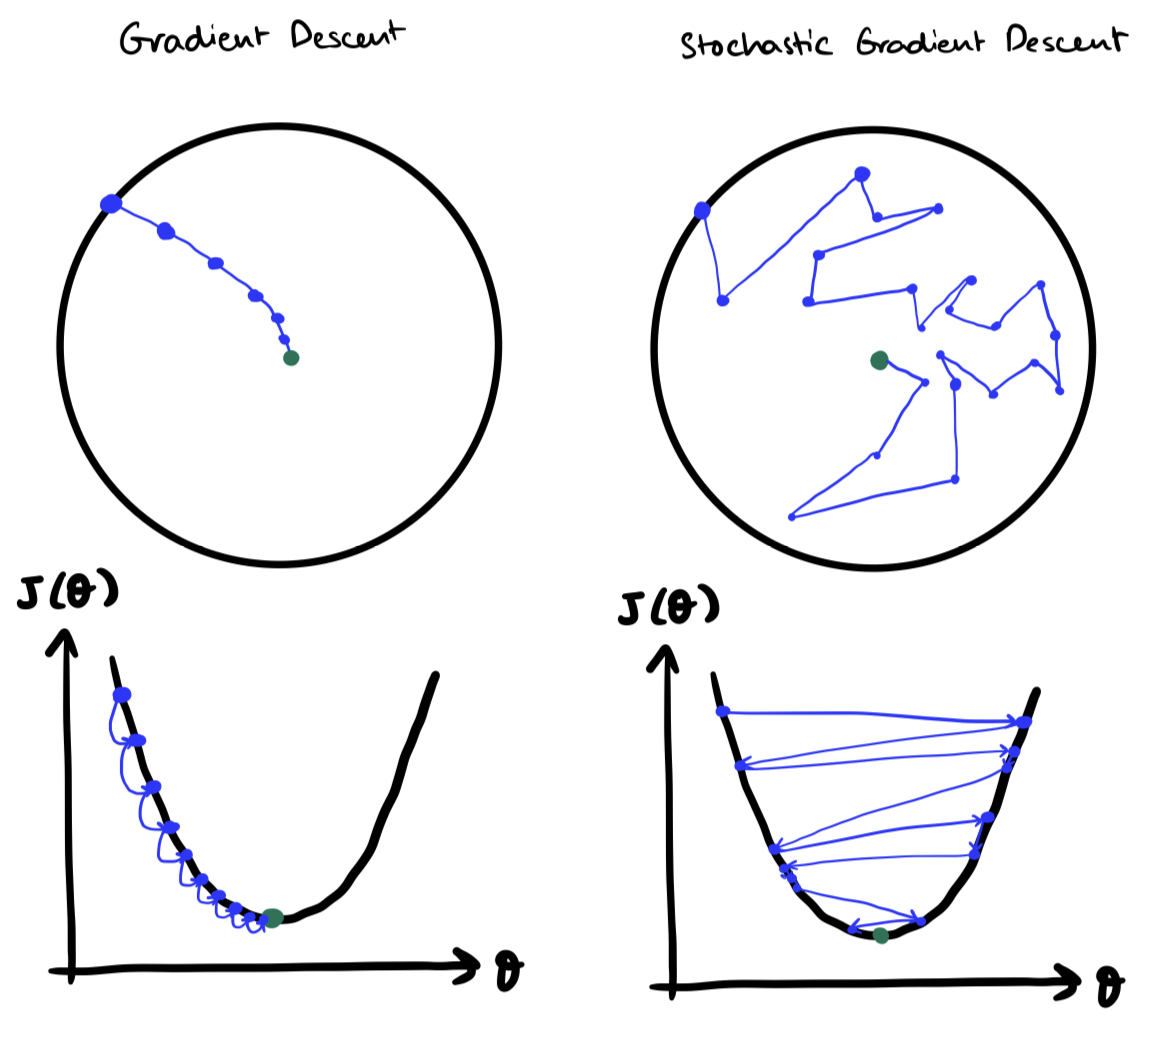
\includegraphics[scale=0.3]{gradient_descent.png}
    \caption{My drawing to show the difference between gradient descent and stochastic gradient descent.}
    \label{gradient-descent}
\end{figure}

\section{Question Two}
\noindent \textbf{What are the four main performance measures (Evaluation Metrics) for the Classification tasks in supervised learning? Explain them in detail with pictures.}

For classification problems, it is necessary to evaluate the model performance. One standard way to measure the performance is through a confusion matrix. Therefore, here is some more terminology before we define the evaluation metrics, which I have also illustrated in Fig. \ref{confusion-matrix}:

\begin{enumerate}
    \item TP (True Positives): how many data points were correctly classified as their real class
    \item FP (False Positives): how many data points were incorrectly classified as another class
    \item FN (False Negatives): how many data points were incorrectly classified as another class
    \item TN (True Negatives): how many data points were correctly classified as another class
\end{enumerate}

This leads us to the four evaluation metrics, defined in terms of the terminology above.

\textbf{Accuracy} is defined as follows: $\frac{TP+TN}{TP+TN+FP+FN}$. The accuracy metric is good for a balanced dataset, and for when every class is important.

\textbf{Precision} is defined as follows: $\frac{TP}{TP+FP}$. The precision metric is good for measuring how often a class is indeed classified correctly, i.e. maximizing on TPs. 

\textbf{Recall} is defined as follows: $\frac{TP}{TP+FN}$. The recall metric is good for measuring how often the other class is indeed classified correctly, i.e. maximizing TNs.

\textbf{F1 Score} is defined as follows: $2\times \frac{precision\times recall}{precision + recall}$. The F1 metric is referred to as a 'harmonic mean between precision and recall'. 

\begin{figure}
    \centering
    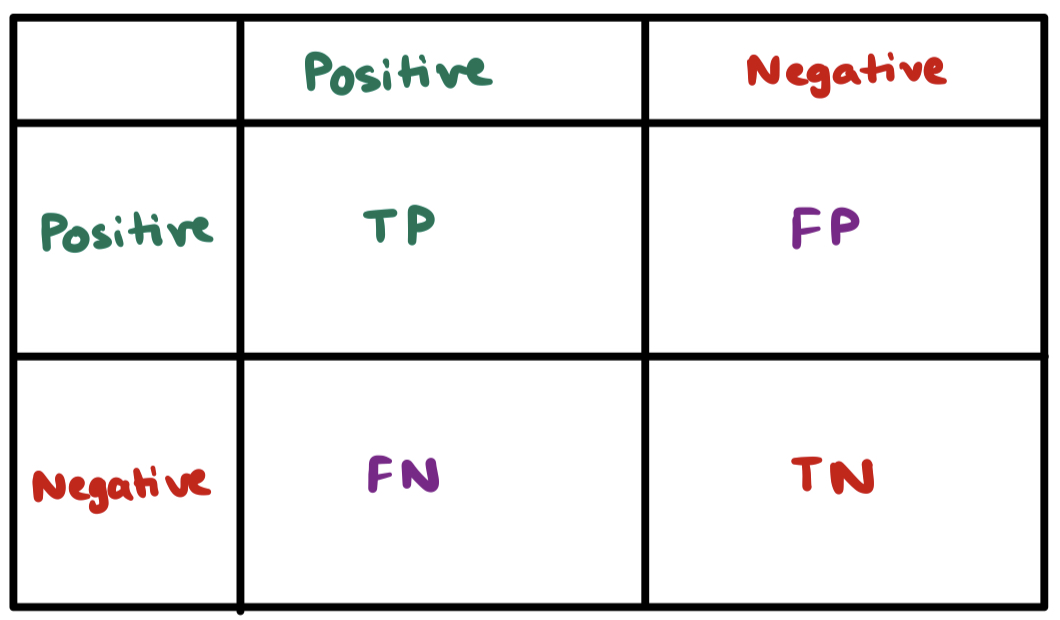
\includegraphics[scale=0.3]{confusion_matrix.png}
    \caption{My drawing to show the confusion matrix.}
    \label{confusion-matrix}
\end{figure}

\section{Question Three}
\noindent \textbf{What is Support vector machine? How are support vectors, decision boundary and margin derived for SVM?}

A Support Vector Machine (SVM) algorithm is a machine learning model that is very powerful in terms of being able to perform linear or nonlinear classification, regression, and outlier detection tasks.

In classification problems, data points are represented as an underlying vector space. A hypersurface divides this vector space into partitions, where each part represents the class of the data points contained within. This hypersurface is called the decision boundary. The space between the decision boundary and the nearest data points is called the margin.

 It uses the kernel trick, which means it transforms data into a higher-dimensional space to make the data linearly separable and hence easier to solve. It builds the classifier with a decision boundary that is furthest from any data point, called support vectors. The margin is the distance between the left and right hyperplanes, i.e. between the support vectors. The support vectors are used to maximize the margin of the classifier, which optimizes the classifier decision boundary.

\section{Question Four}
\noindent \textbf{What are the difference between parameters and hyperparameters? What is a Hyperplane? Use a picture to represent it in 3-dimension space.}

Parameters are internal to the machine learning model, and are learned from the training data. Generally the machine learning training process begins with an initial set of parameters, which could be set to 0 or some constant, or set to random values. The model iterates over the set of initial parameters using an optimization algorithm and updates the parameter set with better values. Finally the set of parameter values at the end of the training process constitute the model.

Hyperparameters are are external to the model, and are set before the machine learning process as inputs to the algorithm. They control the machine learning process to determine how well the algorithm learns the value of the model parameters. These values are fixed and are not changed during the learning process.

A hyperplane is a geometrical vector subspace whose dimension is one less than that of its ambient space. In machine learning, they form decision boundaries to classify data points by dividing the geometrical vector subspace. I have illustrated the hyperplane in Fig. \ref{hyperplane}.

\begin{figure}
    \centering
    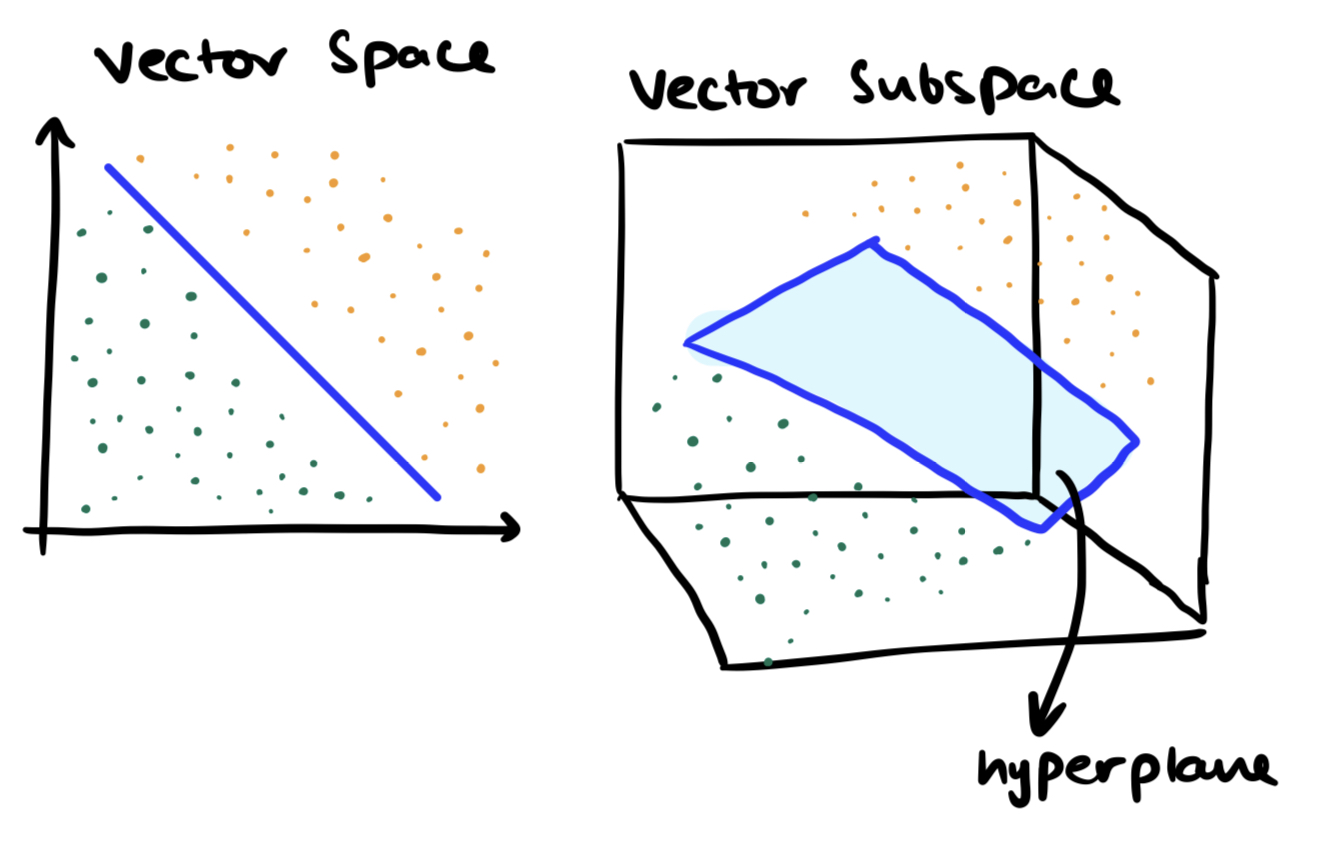
\includegraphics[scale=0.25]{hyperplane.png}
    \caption{My drawing to show a hyperplane.}
    \label{hyperplane}
\end{figure}

\section{Question Five}
\noindent \textbf{What is Feature Engineering and what are different types of Feature Engineering available in Machine Learning?}

Feature engineering is a process to ensure the features in the dataset are the most optimal for the machine learning model. There are different types of feature engineering that can be done.

Feature extraction involves selecting the most relevant features from the raw data, and disregarding irrelevant features, because they are likely to add noise to the model, for example dimensionality reduction, principal components analysis, etc.

Feature transformation involves changing the features in a way that the machine learning model is able to use in a more efficient way, for example scaling, normalization, logarithmic transformations, etc.

Feature creation involves using the existing features to generate new features, for example concatenation, arithmetical operations, etc.

Feature selection involves selecting the most important features, for example based on the relationship between dependent and independent variables, correlation, etc.

Feature engineering can help prevent underfitting/overfitting, and it can also lead to underfitting/overfitting, if it was not done properly. It can also be an iterative process.

\end{document}